This calculator employs an event-based Monte Carlo simulation approach to
probabilistic damage assessment in order to estimate the damage distribution for
individual \glspl{asset} and aggregated damage distribution for a spatially
distributed portfolio of \glspl{asset} within a specified time period. The
calculator requires the definition of an \gls{exposuremodel}, a
\gls{fragilitymodel} for each loss type of interest with
\glspl{fragilityfunction} for each damage state for every typology represented 
in the \gls{exposuremodel}, and a \glsdesc{acr:ses} representative of the 
seismicity of the region over the specified time period. Damage state curves 
and damage maps corresponding to specified return periods can also be 
obtained using this calculator.

As an alternative to computing the \glspl{acr:gmf} with \glsdesc{acr:oqe},
users can also provide their own sets of \glspl{acr:gmf} as input to the
event-based damage calculator.

The main results of this calculator are the event damage tables; these 
tables describe the total number of buildings in each damage state for the
portfolio of \glspl{asset} for each seismic event in the \gls{acr:ses}.

Asset-level event damage tables are generated by the calculator, but are
not exportable in csv format due to the large file sizes that may be
involved. Interested users can access the asset-level event damage tables
within the datastore for the completed calculation.

% Uncomment after the addition of damage curves output
% Damage exceedance curves for each \gls{asset}, which describe 
% the probability of exceedance of different damage levels over the 
% specified time period, and damage maps for the region, which describe the 
% level of damage (for a given damage state) that has a given
% probability of exceedance over the specified time period. Aggregate damage
% exceedance curves can also be produced using this calculator; these
% describe the probability of exceedance of different damage levels for all
% \glspl{asset} in the portfolio.

This calculator relies on the probabilistic event-based hazard calculator,
which simulates the seismicity of the chosen time period $T$ by producing a
\gls{acr:ses}. For each \gls{rupture} generated by a \gls{seismicsource}, the
number of occurrences in the given time span $T$ is simulated by sampling the
corresponding probability distribution as given by $P_{rup}(k | T)$. A
\gls{acr:ses} is therefore a \textit{sample} of the full population of
\glspl{rupture} as defined by a \glsdesc{acr:ssm}. Each \gls{rupture} is
present zero, one or more times, depending on its probability. Symbolically,
we can define a \gls{acr:ses} as:
\begin{align}
SES(T) = \left\{k \times rup,\;k\sim P_{rup}(k | T)\;\;\forall\;rup\;in\;Src\;\forall\;Src\;in\;SSM\right\}
\end{align}
where $k$, the number of occurrences, is a random sample of $P_{rup}(k | T)$,
and $k \times rup$ means that \gls{rupture} $rup$ is repeated $k$ times in the
\gls{acr:ses}.

For each \gls{rupture} or event in the \glspl{acr:ses}, a spatially correlated
\gls{acr:gmf} realisation is generated, taking into consideration both the
inter-event variability of ground motions, and the intra-event residuals
obtained from a spatial correlation model for ground motion residuals (if one 
is specified in the job file). The use of logic trees allows for the 
consideration of uncertainty in the choice of a \glsdesc{acr:ssm}, and in the 
choice of \glspl{groundmotionmodel} for the different tectonic regions.

For each \gls{acr:gmf} realization, a damage state is siumulated for each
building of every \gls{asset} in the \gls{exposuremodel} using the provided
\gls{fragilitymodel}. The asset-level event damage table is saved to the datastore.
Time-averaged damage distributions at the asset-level can be obtained from
the event damage table. Finally damage state exceedance curves can be computed.

The required input files required for running a probabilistic stochastic
event-based damage calculation and the resulting output files are depicted in
Figure~\ref{fig:io-structure-event-based-damage}

\begin{figure}[ht]
\centering
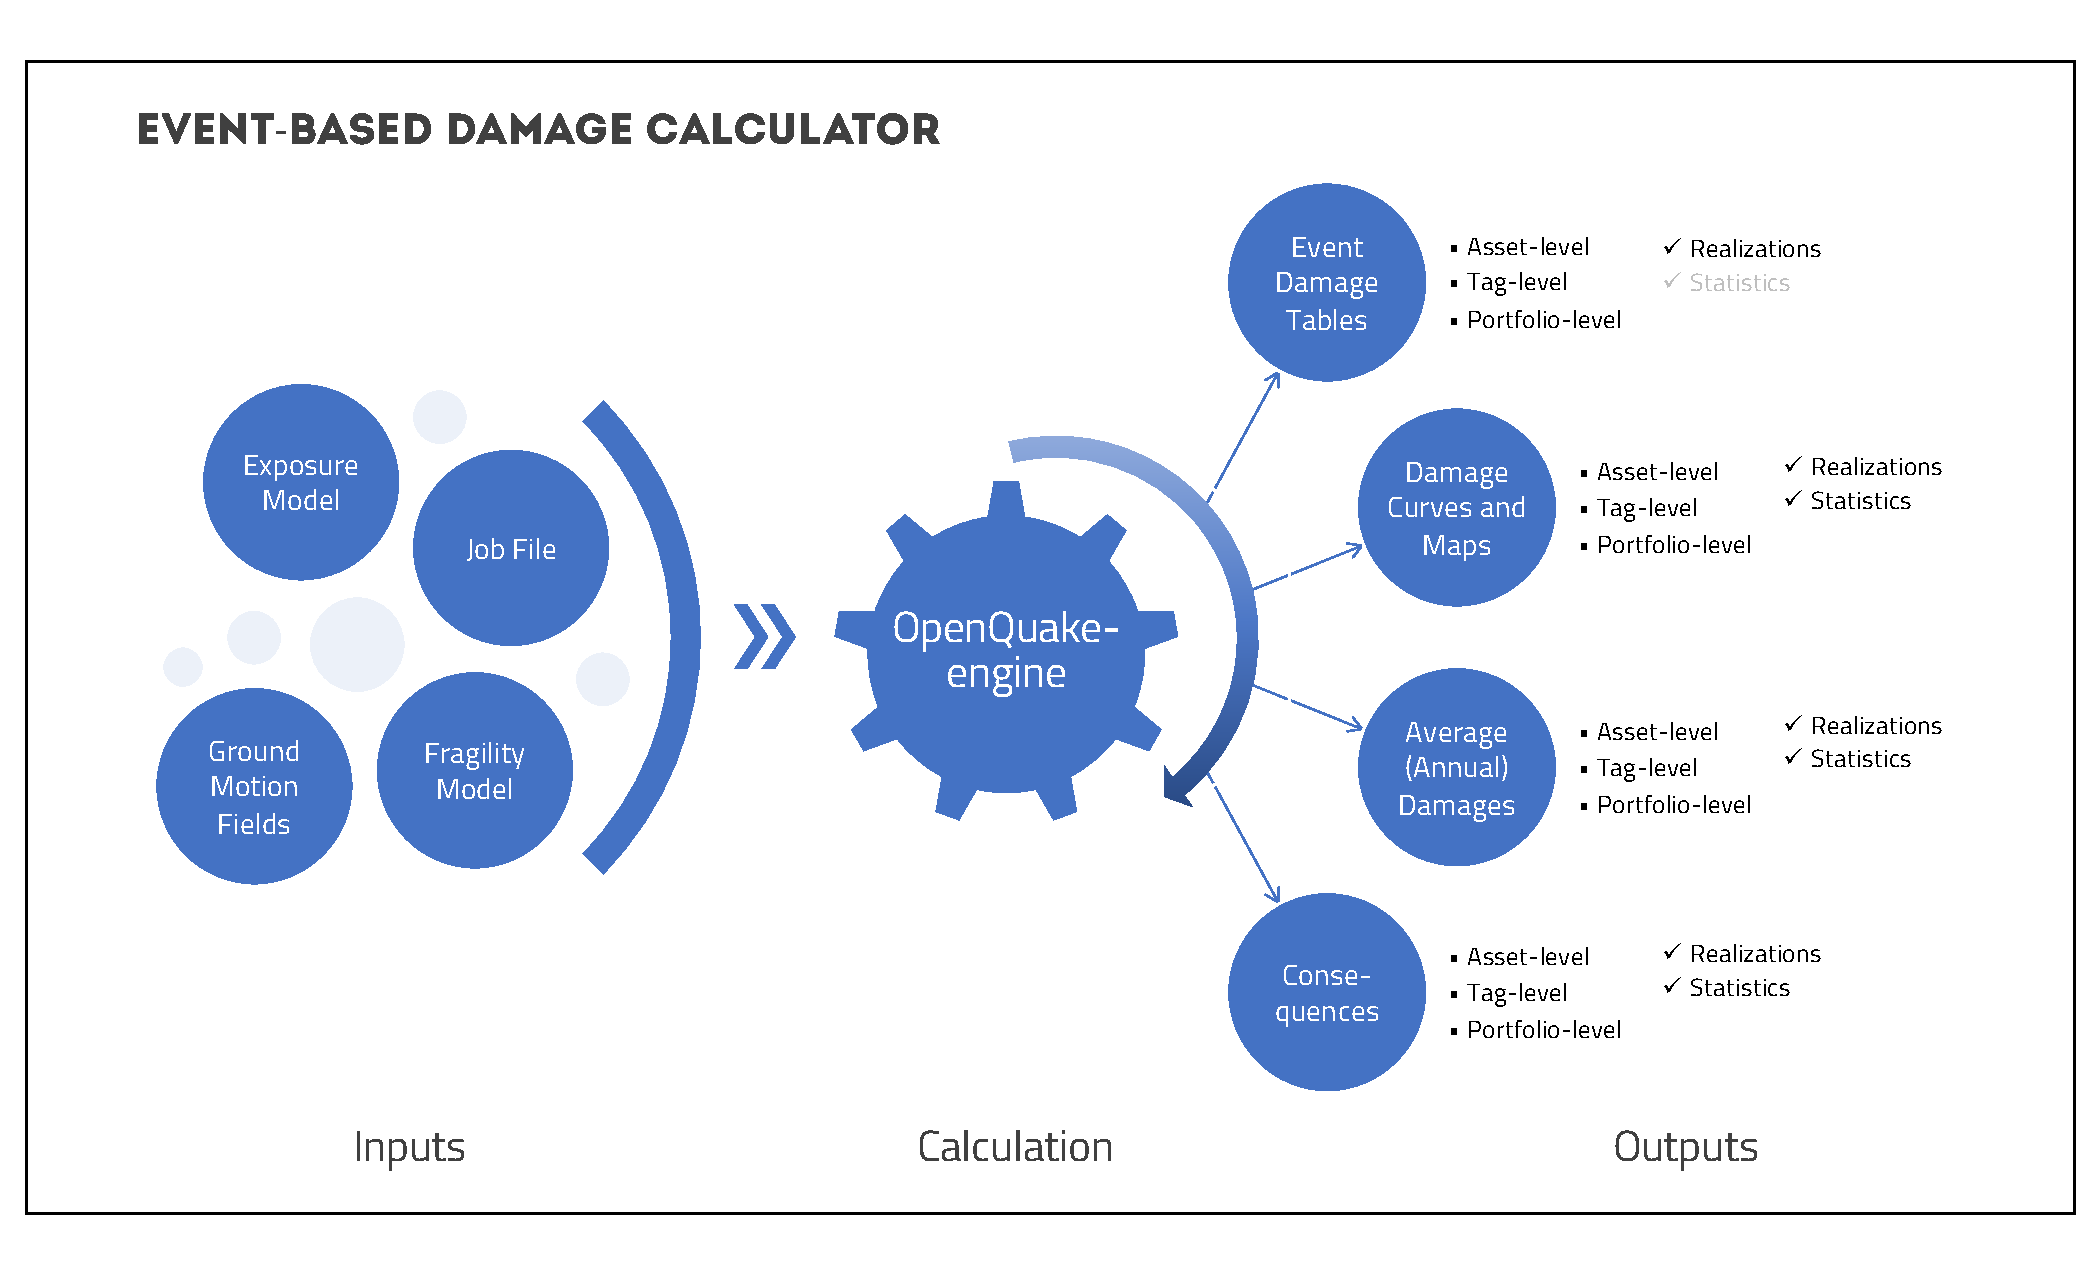
\includegraphics[width=12cm]{figures/risk/io-structure-event-based-damage.pdf}
\caption{Probabilistic Event-based Damage Calculator input/output structure.}
\label{fig:io-structure-event-based-damage}
\end{figure}

Similar to the scenario damage calculator, \gls{consequencemodel} files can also be
provided as inputs for an event-based damage calculation in addition to
\glspl{fragilitymodel} files, in order to estimate consequences based on the
calculated damage distribution. The user may provide one
\gls{consequencemodel} file corresponding to each loss type (amongst
structural, nonstructural, contents, and business interruption) for which a
\gls{fragilitymodel} file is provided. Whereas providing a
\gls{fragilitymodel} file for at least one loss type is mandatory for running
an Event-Based Damage calculation, providing corresponding \gls{consequencemodel}
files is optional.
